\subsection{\label{sec:summary.trigger}Trigger Configurations}

\begin{center} \color{OliveGreen}
This section is a verbatim excerpt from the dissertation by J.T.\ Goetz\cite{clas.thesis.goetz}.
\end{center}

The \desg{g12} experiment was the first Hall \desg{B} run-period to implement field programmable gate array (\abbr{FPGA}) processors to handle the trigger logic of the \abbr{abbr{CLAS}} detector (see Sec.~\ref{sec:clas.daq}). With this new \abbr{FPGA}-powered triggering system, came the ability to modify the trigger quickly during the experiment. While potentially dangerous --- these changes must be accounted for in total-cross-sectional analyses for example --- this allowed the group to tune the trigger to get the highest possible rate of physical events.

The trigger bits used during the \desg{g12} running period are defined in Tables~\ref{tab:data.trig.conf.1}, \ref{tab:data.trig.conf.2} and \ref{tab:data.trig.conf.3}. They generally consisted of a number of tracks which were the coincidence of any one of the four start counter paddles and any of the 57 time-of-flight paddles in a given sector as discussed in Sec.~\ref{sec:clas.daq}. The hardware and configuration did not allow triggering on two tracks in the same sector because there were only six signals coming from the \abbr{TOF} --- one for each sector. The coincidence of these tracks with the photon tagger, called the ``Master-\abbr{OR},'' is defined in Table~\ref{tab:data.trig.mor}.

\begin{table}
\begin{minipage}{\textwidth}
\begin{center}
\begin{singlespacing}

\caption[Trigger Configuration 1]{\label{tab:data.trig.conf.1}Trigger configuration for \desg{g12} runs from 56363 to 56594 and 56608 to 56647. (\abbr{ST}$\times$\abbr{TOF})$_{i}$ indicates a single \emph{prong} which is a trigger-level track defined as a coincidence between a start counter and time-of-flight hit in the \ith\ sector or any sector if the subscript index, $i$, is not specified. An added $\times$2 or $\times$3 indicates the coincidence of multiple \emph{prongs} which are not in the same sector. \abbr{MORA} and \abbr{MORB} represent coincidences with tagger hits within a certain energy range as specified in Table~\ref{tab:data.trig.mor}.}

\begin{tabular}{cccc}

\hline \hline

\multicolumn{4}{c}{\desg{g12} runs 56363--56594, 56608--56647} \\

\hline

bit & definition & L2 multiplicity & prescale \\

\hline

1 & \abbr{MORA}$\cdot$(\abbr{ST}$\times$\abbr{TOF})$_{1}\cdot$(\abbr{ST}$\times$\abbr{TOF}) & -- & 1 \\
2 & \abbr{MORA}$\cdot$(\abbr{ST}$\times$\abbr{TOF})$_{2}\cdot$(\abbr{ST}$\times$\abbr{TOF}) & -- & 1 \\
3 & \abbr{MORA}$\cdot$(\abbr{ST}$\times$\abbr{TOF})$_{3}\cdot$(\abbr{ST}$\times$\abbr{TOF}) & -- & 1 \\
4 & \abbr{MORA}$\cdot$(\abbr{ST}$\times$\abbr{TOF})$_{4}\cdot$(\abbr{ST}$\times$\abbr{TOF}) & -- & 1 \\
5 & \abbr{MORA}$\cdot$(\abbr{ST}$\times$\abbr{TOF})$_{5}\cdot$(\abbr{ST}$\times$\abbr{TOF}) & -- & 1 \\
6 & \abbr{MORA}$\cdot$(\abbr{ST}$\times$\abbr{TOF})$_{6}\cdot$(\abbr{ST}$\times$\abbr{TOF}) & -- & 1 \\
7 & \abbr{ST}$\times$\abbr{TOF} & -- & 1 \\
8 & \abbr{MORA}$\cdot$(\abbr{ST}$\times$\abbr{TOF})$\times$2 & -- & 1 \\
11\footnote{bit 11 and \abbr{MORB} were included in the trigger starting with run 56519.} & \abbr{MORB}$\cdot$(\abbr{ST}$\times$\abbr{TOF})$\times$2 & -- & 1 \\
12 & (\abbr{ST}$\times$\abbr{TOF})$\times$3 & -- & 1 \\

\hline \hline

\end{tabular}

\end{singlespacing}
\end{center}
\end{minipage}
\end{table}
 % label: tab:data.trig.conf.1

\begin{table}
\begin{minipage}{\textwidth}
\begin{center}
\begin{singlespacing}

\caption[Trigger Configuration 2]{\label{tab:data.trig.conf.2}Trigger configuration for \desg{g12} runs from 56595 to 56607 and 56648 to 57323. (\abbr{EC}$\times$\abbr{CC}) represents a coincidence between the electromagnetic calorimeter and the \v{C}erenkov subsystems within a single sector using the thresholds as described in Table~\ref{tab:data.ecccthresh}. \abbr{ECP} represents the \emph{photon} threshold trigger from the \abbr{EC} as detailed in Fig.~\ref{fig:clas.daq.trigsec}. See Table~\ref{tab:data.trig.conf.1} for other explanatory details.}

\begin{tabular}{cccc}

\hline \hline

\multicolumn{4}{c}{\desg{g12} runs 56595--56607, 56648--57323 } \\

\hline

bit & definition & L2 multiplicity\footnote{Level 2 triggering was turned off on all bits for runs 56605, 56607 and 56647.} & prescale \\

\hline

1 & \abbr{MORA}$\cdot$(\abbr{ST}$\times$\abbr{TOF}) & 1 & 1000/300\footnote{Prescaling for bits 1 and 4 were 1000 for runs prior to 56668 at which point they both were changed to 300.} \\
2 & \abbr{MORA}$\cdot$(\abbr{ST}$\times$\abbr{TOF})$\times$2 & 2/--\footnote{Level 2 triggering of bit 2 was set to 2 for runs prior to 56665 at which point it was turned off.} & 1 \\
3 & \abbr{MORB}$\cdot$(\abbr{ST}$\times$\abbr{TOF})$\times$2 & 2 & 1 \\
4 & \abbr{ST}$\times$\abbr{TOF} & 1 & 1000/300 \\
5 & (\abbr{ST}$\times$\abbr{TOF})$\cdot$\abbr{ECP}$\times$2 & 1 & 1 \\
6 & (\abbr{ST}$\times$\abbr{TOF})$\cdot$(\abbr{EC}$\times$\abbr{CC}) & 2 & 1 \\
7 & \abbr{MORA}$\cdot$(\abbr{ST}$\times$\abbr{TOF})$\cdot$(\abbr{EC}$\times$\abbr{CC}) & -- & 1 \\
8 & \abbr{MORA}$\cdot$(\abbr{ST}$\times$\abbr{TOF})$\times$2 & -- & 1 \\
11 & (\abbr{EC}$\times$\abbr{CC})$\times$2 & -- & 1 \\
12 & (\abbr{ST}$\times$\abbr{TOF})$\times$3 & -- & 1 \\

\hline \hline

\end{tabular}

\end{singlespacing}
\end{center}
\end{minipage}
\end{table}

 % label: tab:data.trig.conf.2

\begin{table}
\begin{minipage}{\textwidth}
\begin{center}
\begin{singlespacing}

\caption[Trigger Configuration for Single-sector Runs]{\label{tab:data.trig.conf.3}Trigger configuration for the single-sector runs of \desg{g12}. Trigger bits 7--12 were not used for these runs. See Table~\ref{tab:data.trig.conf.1} for explanatory details.}

\begin{tabular}{cccc}

\hline \hline

bit & definition & L2 multiplicity & prescale \\

\hline

1 & \abbr{MORA}$\cdot$(\abbr{ST}$\times$\abbr{TOF})$_{1}$ & sector 1 & 1 \\
2 & \abbr{MORA}$\cdot$(\abbr{ST}$\times$\abbr{TOF})$_{2}$ & sector 2 & 1 \\
3 & \abbr{MORA}$\cdot$(\abbr{ST}$\times$\abbr{TOF})$_{3}$ & sector 3 & 1 \\
4 & \abbr{MORA}$\cdot$(\abbr{ST}$\times$\abbr{TOF})$_{4}$ & sector 4 & 1 \\
5 & \abbr{MORA}$\cdot$(\abbr{ST}$\times$\abbr{TOF})$_{5}$ & sector 5 & 1 \\
6 & \abbr{MORA}$\cdot$(\abbr{ST}$\times$\abbr{TOF})$_{6}$ & sector 6 & 1 \\

\hline \hline

\end{tabular}

\end{singlespacing}
\end{center}
\end{minipage}
\end{table}

 % label: tab:data.trig.conf.3

\begin{table}
\begin{center}
\begin{singlespacing}

\caption[Trigger Configuration (Tagger)]{\label{tab:data.trig.mor}Master-\abbr{OR} definitions for \desg{g12}. The \abbr{TDC} counters were used in the trigger and since each of these corresponds to several energy paddles, the energies given here are approximate. $T$-counter number 1 corresponds to the highest energy photon of approximately 5.4~GeV. Both \abbr{MORA} and \abbr{MORB} are referenced in terms of the trigger logic in Tables~\ref{tab:data.trig.conf.1}, \ref{tab:data.trig.conf.2} and \ref{tab:data.trig.conf.3}. The \emph{single-sector} runs are listed in Table~\ref{tab:data.cook.singlesecruns}.}

\begin{tabular}{c|cc|cc}

\hline \hline

          & \multicolumn{2}{c|}{\abbr{MORA}} & \multicolumn{2}{c}{\abbr{MORB}} \\
run range & $T$-counters & energy (GeV)     & $T$-counters & energy (GeV) \\

\hline

56363--56400 & 1--47 & 1.7--5.4 & -- & -- \\
56401--56518 & 1--25 & 3.6--5.4 & -- & -- \\
56519--57323 & 1--19 & 4.4--5.4 & 20--25 & 3.6--4.4 \\

\hline

\emph{single-sector} & 1--31 & 3.0--5.4 & -- & -- \\

\hline \hline

\end{tabular}

\end{singlespacing}
\end{center}
\end{table}
 % label:  tab:data.trig.mor

There were two sets of thresholds for the \abbr{EC} labeled \emph{photon} and \emph{electron}. These labels did not mean photon or electron specifically, but were considered a first-order approximation. The actual particle identification was done much later in the analysis of the reconstructed data. The thresholds for the \abbr{CC} and \abbr{EC} during the \desg{g12} running period are shown in Table~\ref{tab:data.ecccthresh}.

\begin{table}
\begin{center}
\begin{singlespacing}

\caption[\abbr{EC} and \abbr{CC} Trigger Thresholds]{\label{tab:data.ecccthresh}Threshold values for the electromagnetic calorimeter (\abbr{EC}) and \v{C}erenkov counter (\abbr{CC}) during the \desg{g12} running period. \abbr{EC} thresholds are shown as \emph{inner}/\emph{total}, and \abbr{CC} thresholds are shown as \emph{left}/\emph{right}.}

\begin{tabular}{cc|c}

\hline \hline

\multicolumn{2}{c|}{\abbr{EC}} & \multirow{2}{*}{\abbr{CC}} \\

\emph{photon} & \emph{electron} \\


\hline

50/100~mV & 60/80~mV & 20/20~mV \\
150/300~MeV & 180/240~MeV & $\sim$0.4~photo-electrons \\

\hline \hline

\end{tabular}

\end{singlespacing}
\end{center}
\end{table}
 % label: tab:data.ecccthresh

\subsection{\label{sec:data.trig.eff}Trigger Efficiency Study}

\begin{center} \color{OliveGreen}
This section is a verbatim excerpt from the dissertation by J.T.\ Goetz\cite{clas.thesis.goetz}.
\end{center}

In the first few weeks of \desg{g12}, during ``commissioning,'' an attempt to determine the efficiency of the two-track trigger (bit 8 in Tables.~\ref{tab:data.trig.conf.1} and \ref{tab:data.trig.conf.2}) was made. The rate of this main production trigger rose quadratically with the beam current while the physical event rate increased linearly. The number of accidentals, which must be cut from any analysis, increased with increasing current and at a certain point, the majority of the events taken were accidentals. The trigger rate as a function of the beam current is shown in Fig.~\ref{fig:data.trig.eff}. An estimate of the linear part of the trigger rate shows that approximately 60\% of the events recorded during the \desg{g12} experiment (which ran at 60--65~nA beam current) were accidentals.

\begin{figure}\begin{center}
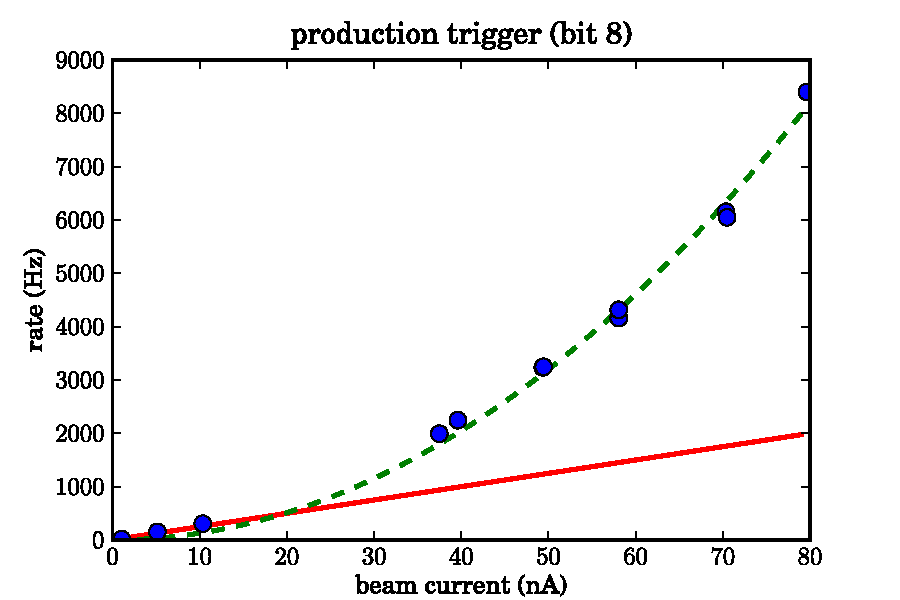
\includegraphics[width=0.7\columnwidth]{figures/calib/trig/trigger_study.eps}
\caption[Trigger Rate vs. Beam Current]{\label{fig:data.trig.eff}The production trigger rate (bit 8 in Tables~\ref{tab:data.trig.conf.1} and \ref{tab:data.trig.conf.2}) was measured for various beam currents shown by the blue dots. The rates below 10~nA are roughly linear and are extrapolated via the red solid line to show an estimate of the physical event rate. The actual trigger rate is fitted with a quadratic shown by the green dashed line. By this estimate, the accidental rate is shown to equal the physical event rate at approximately 40~nA. The \desg{g12} experiment was done at 60--65~nA.}
\end{center}\end{figure}

\clearpage
